% \documentstyle[amssymb,12pt,draft,epsf,palatino]{nature-pvd}
\documentclass{natureprintstyle}
\bibliographystyle{naturemag}

\usepackage{epsfig,caption}
\usepackage{color}
\usepackage{bm}
\usepackage{graphicx}
\usepackage{longtable}
\usepackage{amssymb}
\usepackage{rotating,xcolor}
\usepackage{hyperref}
\hypersetup{
    colorlinks,
    linkcolor={blue!50!black},
    citecolor={blue!80!white},
    urlcolor={blue!80!black}
}

\renewcommand{\floatpagefraction}{.9}

\newcommand{\msun}{\ensuremath{\textrm{M}_\odot}}
\newcommand{\gyr}{\ensuremath{\textrm{Gyr}}}
\newcommand{\kpc}{\ensuremath{\textrm{kpc}}}
\newcommand{\mas}{\ensuremath{\textrm{mas}}}
\newcommand{\ul}{\ensuremath{\textrm{kpc}^2\,\textrm{Myr}^{-1}}}
\newcommand{\ue}{\ensuremath{\textrm{kpc}^2\,\textrm{Myr}^{-2}}}
\newcommand{\kms}{\ensuremath{\textrm{km}\,\textrm{s}^{-1}}}
\newcommand{\masyr}{\ensuremath{\textrm{mas}\,\textrm{yr}^{-1}}}
\newcommand{\feh}{\ensuremath{\textrm{[Fe/H]}}}
\newcommand{\afe}{\ensuremath{\textrm{[$\alpha$/Fe]}}}

\newcommand{\package}[1]{\textsl{#1}}

\title{\huge Sagittarius merger rippling the entire Milky Way galaxy}
% \title{Signatures of long-lived ripples throughout the Milky Way galaxy}

\author{Ana Bonaca$^1$, Rohan P. Naidu$^{2,3}$, Charlie Conroy$^4$}

\begin{document}

\maketitle
\let\thefootnote\relax\footnote{

\begin{affiliations}
\item The Observatories of the Carnegie Institution for Science, Pasadena, CA, USA
\item Massachusetts Institute of Technology, Cambridge, MA, USA
\item Hubble Fellow
\item Center for Astrophysics $|$ Harvard \& Smithsonian,  Cambridge, MA, USA
% \item Steward Observatory, University of Arizona, 933 North Cherry Avenue, Tucson, AZ 85721, USA
\end{affiliations}
}

\vspace{-3.5mm}
\begin{abstract}
Mergers are driving the formation of galaxies like the Milky Way: they build up the stellar and dark-matter mass (cit), as well as affect existing structures (cit).
These perturbations are longest-lived off of the plane (cit), but our precise measurements of the dynamical orbital space have so far been confined to the Solar neighborhood, and therefore only uncovered the most recent perturbations (cit), rather than their entire cosmic history.
Here we report a spectrum of orbital resonances in a sample of nearly 20,000 giant stars beyond the Galactic disk plane as nearly equidistant peaks in orbital energies on both disk- and halo-like orbits.
Using numerical experiments we show that the accretion of the Sagittarius dwarf galaxy can form such ripples, with the ripple strength being set by the mass of the merger, while their positions depend on its orbital history.
The orbital decay, sensitive to the nature of dark matter, of any merger has not been reconstructed despite this being the key way that galaxies grow
Matching the narrow energy spacing between the ripples requires modeling the effects of dynamical friction and mass-loss.
Assuming Chandrasekhar dynamical friction(cit) and a linear mass loss, we find that Sagittarius lost $99\%$ of its total mass, consistent with CDM predictions (cit).
The mass-loss rates of dark-matter halos depend sensitively on their density profile, so the detected ripples provide a unique constraint on the particle nature of dark matter.
% - and a sensitive test of the particle nature of dark matter (predict different density profiles, and therefore mass-loss histories)
% %
% Galaxies and their dark-matter halos grow through accretion of smaller galaxies (theory cit), which has been abundantly documented in the Milky Way.
% - MW mergers driving galaxy formation: building up stellar mass + dm mass %+ perturbing the existing structures
% - former abundantly observed in the MW, and latter as recent perturbations in the phase-space of nearby stars % combine in first sentence
% While the- hard beyond the last Gyr due to signatures being erased in the disk / Solar neighborhood, but longer-lived beyond (cite)
% Most recent perturbations visible in the Solar neighborhood (cit), but longer-lived away from the plane and scattering off of spiral arms and giant molecular clouds (cit).
% - Sgr merger -- standard for calibrating tidal disruption of a dark-matter subhalo, 
% - however, slight mis-match, especially at higher energies -- potentially non-linear mass-loss history
%%
% - evidence in the MW disk of recent perturbation, but older history erased
% and identify them as Sgr ripples
% Using a sample of $\sim20,000$ old, giant stars beyond the Milky Way's disk plane ($|Z_{gal}|\gtrsim2$\,kpc), we find evidence of discrete orbital resonances at constant orbital energies.
% The resonances ubiquitous, are present throughout the Galaxy, both in the high-latitude disk and in the radial halo -- first time 
% % - at same locations, also in different parts of the Galaxy.
% - recent mw in disequilibrium: possible sources of perturbation: internal -- bar, external -- satellite merger
% - through a series of numerical experiments, we demonstrate that a perturbation by a massive satellite, like the Sagittarius dwarf galaxy, is needed to excite the observed resonances
% - the amplitudes of the peaks is related to the mass of the perturber, while their energy levels are determined by the past orbit of the satellite
% - we find that a massive Sgr, w mass-loss, produces the observed resonances
% - dynamical friction + mass-loss crucial elements to match the resonant energies, tidal stripping, first time we can directly measure it -- potential for DM microphysics 
% - satellite tidal stripping relevant for cosmology more broadly? (check w Andrew)
% % - orbital history largely depends on , mapping of these resonances will allow reconstruction of Sgr past orbit
% - mergers are agents of chaos, but there is also regularity + information
% % (- check in sims / data if features more informative beyond the plane)
% % - measure where the peaks are
% % - kick off industry to constrain the locations of the peaks (test using chervin's models? share a notebook w the H3 selection function, potential we used)
\end{abstract}
% \vspace{0.5cm}

%%%%%%%%%%%%%%%%%%%%%%%%%%%%%%%%%%%%%%%%%%%%%%%%%%%%%

\begin{figure*}
\begin{center}
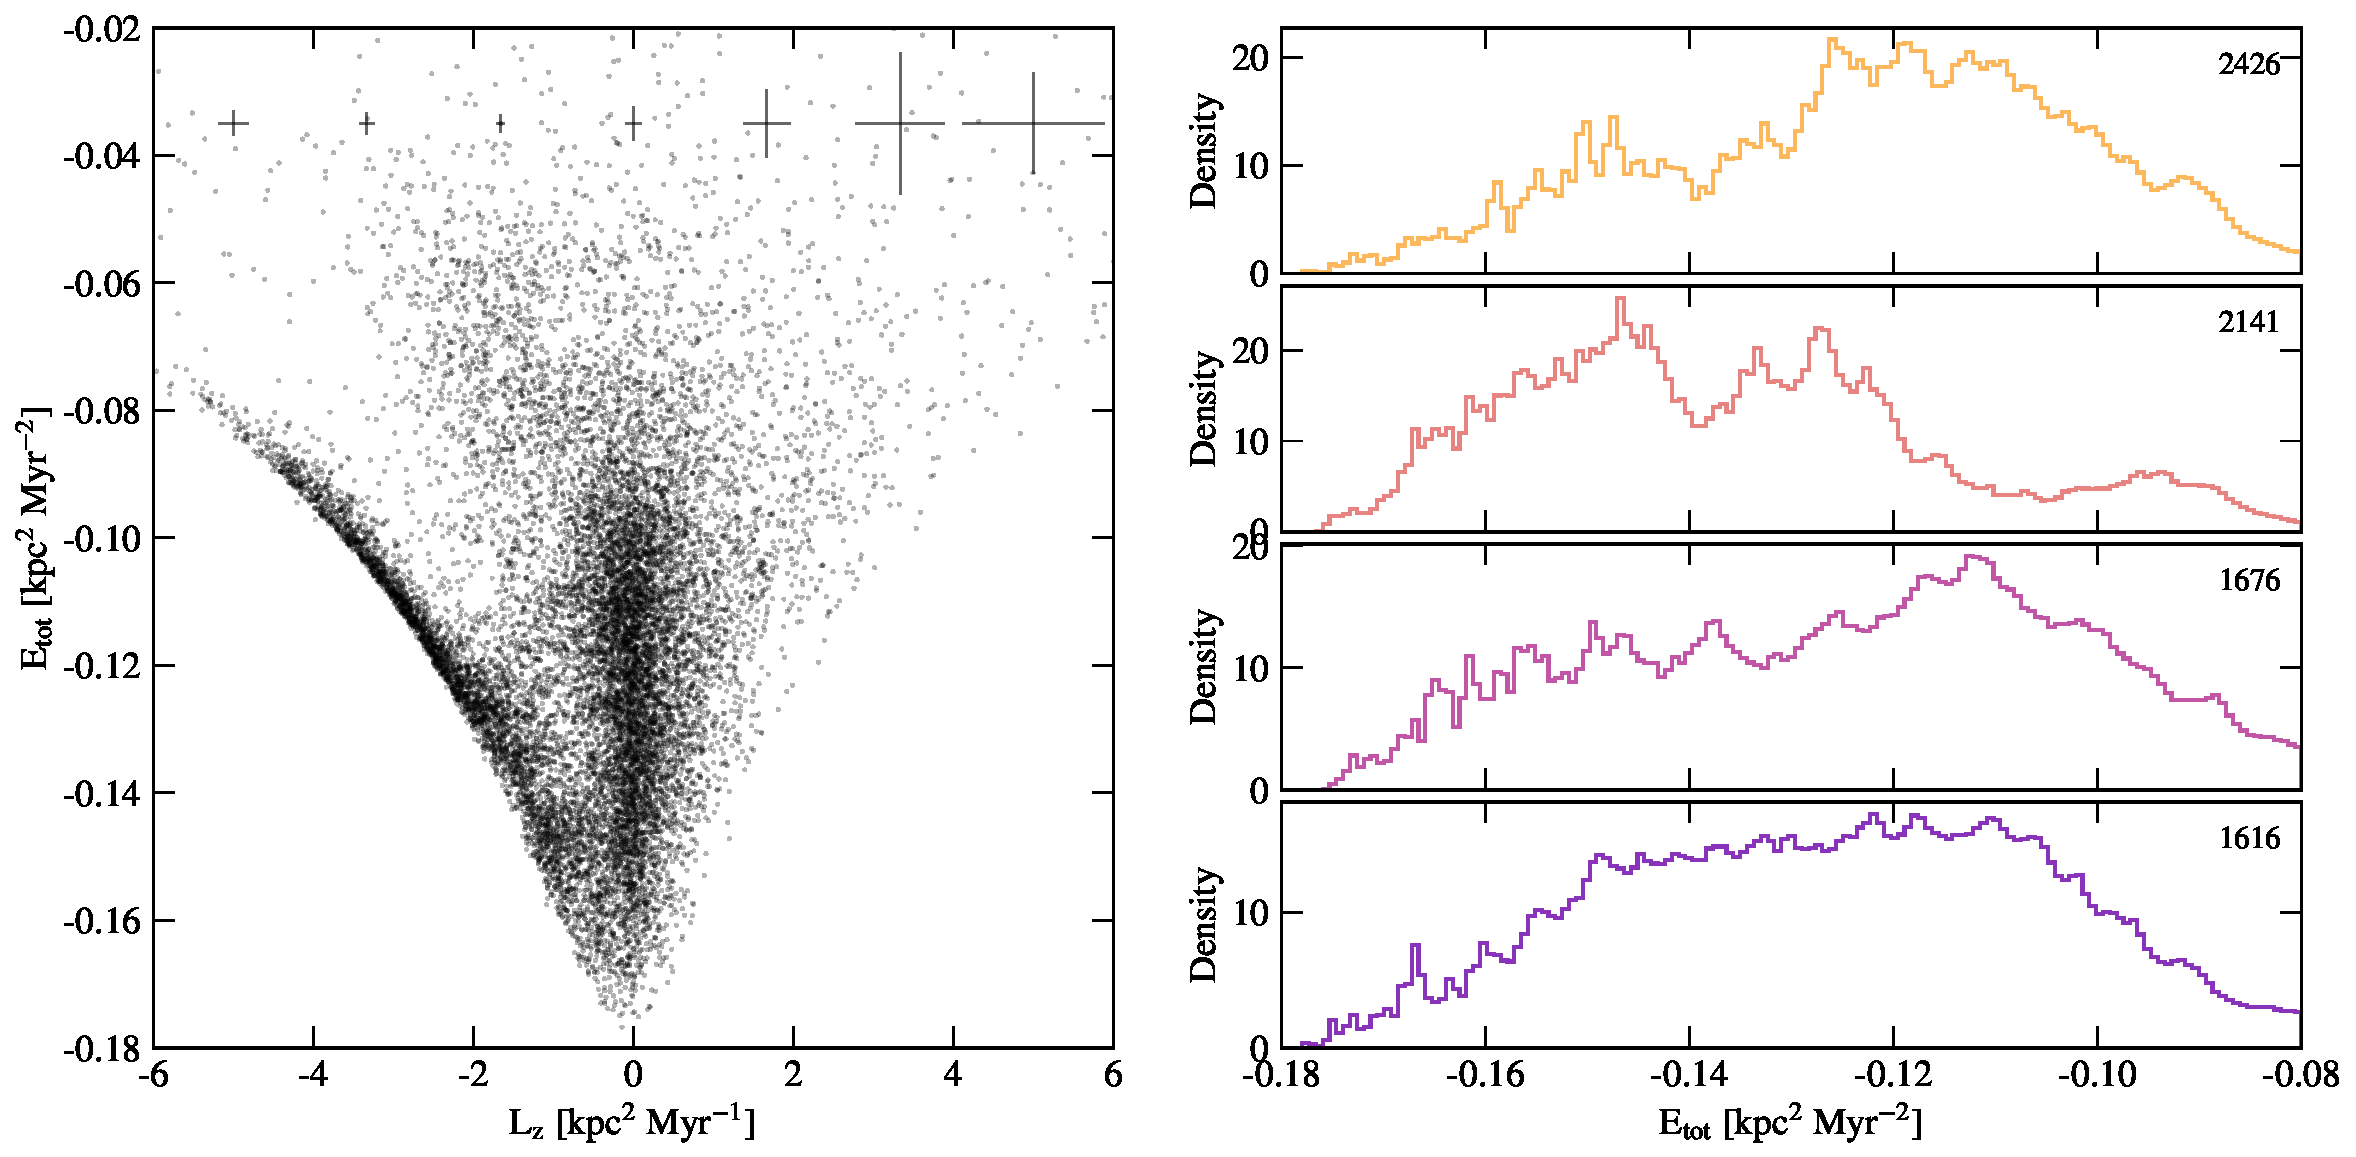
\includegraphics[width=0.99\textwidth]{fig1.pdf}
\vspace{-4mm}
\caption{\small
\textbf{Orbital phase-space of Milky Way stars.}
{\bf Left:} Total orbital energies as a function of the $z$ component of orbital angular momentum (perpendicular to the Milky Way disk) of stars in the H3 survey.
Typical measurement uncertainties are shown as errorbars on top as a function of angular momentum.
- ripples
{\bf Right:} Distributions of orbital energies for disk (top) and halo (bottom) stars show a spectrum of orbital resonances at constant energy.
- best-fit model
}
\vspace{-4mm}
\label{fig:elz}
\end{center}
\end{figure*}

We used optical spectroscopy from the ``Hectochelle in the Halo at High-resolution'' (H3) survey\cite{conroy:2019} to select $\approx20,000$ giant stars ($\log g<3.5$, where $g$ is surface gravity) and precisely map the orbital phase-space beyond the Milky Way disk plane (the H3 survey targets are located at high Galactic latitudes, $|b|>30^\circ$, and between 2\,kpc and 100\,kpc from the Sun).
The H3 data reduction pipeline\cite{cargile:2020} combines these spectra with optical through infrared photometry, and for this sample measures extremely precise radial velocities and distances (90-th percentile uncertainties of $0.5\,\kms$ and 14\%, respectively).
Using proper motions from the Gaia Data Release 3\cite{gaiaedr3}, and adopting the \package{astropy}~v4.1 solar position\cite{astropy:2022} and \package{gala}~\package{MilkyWayPotential2022} gravitational potential model\cite{gala}, we calculated 3D positions and 3D velocities for these stars, as well as their orbital energies, $E_{tot}$, and angular momenta with respect to the disk plane, $L_z$.

The energy--angular momentum phase space of H3 giants is shown in the left panel of Figure~\ref{fig:elz}.
Since these quantities are nearly-conserved through the cosmic history, stars of common origin have been identified as phase-space clusters: thick disk stars as the left envelope, the Gaia-Sausage-Enceladus merger\cite{belokurov:2018,helmi:2018} at $L_z\approx0$, Sequoia merger\cite{myeong:2019,naidu:2020} on the right, and tidal debris of the Sagittarius (Sgr) dwarf galaxy\cite{ibata:2001,johnson:2020} at top left.
Thanks to the exquisite precision of the recovered orbital parameters (typical uncertainties are shown at the top), these data also reveal substructure in the two major components: a series of ripples at constant density both in the disk (marked with orange arrows) and in the GSE merger (blue arrows).

Right panels of Figure~\ref{fig:elz} show energy histograms for groups of stars with the most prominent ripples: eccentric thick-disk stars (top, $0.35<circ<0.7$, $L_z<0$) and prograde GSE halo stars (bottom, $0.7<ecc<0.9$, $L_z<0$).
- rippled wrt smooth mock (rybizki)
- measure peaks on KDE (bandwidth 0.05, approx width of the peaks) -- details in methods
- number of prominent peaks (some number of sigma above background, defined somehow)
- within uncertainties, same positions in the disk and the halo
- approximately uniformly spaced by yy $kpc^2 Myr^{-2}$ or $(xx km/s)^2$
% - fit mixture of gaussians
% - auxiliary materials: non-bootstrapped version, function of snr; number of components

Phase-space structures like energy ridges naturally form in merging tidal debris\cite{gomez:2010, gomez:2012a, belokurov:2023}.
However, given that we detected ripples at the same energies in two populations of stars with different kinematics, chemistry and origin---the disk and the halo---implies they have been formed through a global dynamical perturbation.
Structures massive enough to dynamically perturb stars in the radial range $5\,\kpc\lesssim r \lesssim 30\,\kpc$ (see appendix for spatial coverage of our sample) are a rotating bar, or a massive merger event.
A galactic bar is extremely effective in trapping stars orbiting in resonance close to the disk plane\cite{dehnen:2000, trick:2021, dilamore:2023}, but our numerical experiments (appendix) show that above the plane these are weaker, leaving the merger scenario as the sole viable origin for the ripples.

% - alternative: distinct accretion events
% - smaller accretion events present, not obvious as overdensities\cite{naidu:2020}
% - test through chemistry -- largely the same

Sagittarius is the only prominent merger the Milky Way experienced after the formation of the thick disk and the GSE merger and could affect both components\cite{ruiz-lara:2020, kruijssen:2020, bonaca:2020}.
We ran idealized N-body experiments to explore whether a Sagittarius-like merger can form the observed phase-space ripples in the Milky Way.
The merging satellite was initialized at the present-day position of Sagittarius\cite{vasiliev:2021} as a Hernquist sphere\cite{hernquist:1990} with a mass of $1\times10^{10}\,\msun$, comparable to the massive Sagittarius models\cite{laporte:2018}.
Our Milky Way model has two components: (i) 100,000 disk particles, initialized to form a self-consistent thick disk, with properties typical of a $z=2$ disk, and the velocity scale adjusted to match the Milky Way today, and (ii) 50,000 halo particles, initialized as the final N-body snapshot of a GSE-like debris\cite{naidu:2021}.
Sagittarius and all of the Milky Way particles were evolved for 6\,Gyr in a three-component, static background potential\cite{gala:2022}.

- what's happening
- looks like 
- sensitive to orbital history
- needs dynamical friction + mass-loss to reproduce energy spacing
- quantification: x/xx most-prominent peaks matched?

% - describe fig 2: peaks measure the total orbital history
% - what do peaks correspond to in relation to Sgr orbit?
% - examples of no mass-loss, best-fit, too much

- exciting that we are sensitive to mass-loss: depends directly on the mass profile of the dwarf
- encodes dm physics, but long-standing question, hard to observe directly
- more broadly orbital decay most fundamental process in astrophysics -- Sgr can serve as standard for calibration

- implications for MW: recent perturbations seen recently in the Solar neighborhood, origin still unclear
- can disentangle Sgr from other effects
- comment on Helmer's work seeing Sgr resonances?

- limitations + next steps
- idealized Sgr models -- great that CDF works + matches most peaks, there are deviations at high energies, especially in the halo
- current modeling just an approximation, so should do better and get a full picture in comparison w self-consistent N-body sims (cit Hunt, Chervin?)

% - discrepancies
% - comparison to other perturbations

% - what we'll learn from this
% -- subhalo survival related to expected dm annihilation rates)
% -- vdbosch: Accurately predicting the demographics of dark matter (DM) substructure is of paramount importance for many fields of astrophysics, including gravitational lensing, galaxy evolution, halo occupation modelling, and constraining the nature of DM.
% -- so far, dm tidal disruption only theoretical, plagued by resolution issues
% -- here empirical!

%%%%%%%%%%%%%%%%%%%%%%%%%%%%%%%%%%%%%%%%%%%%%%%%%%%%

% \bibliographystyle{naturemag}
{\small\bibliography{references}}

\begin{addendum}
  
\item [Acknowledgements] 
% We thank both referees for their constructive
%   feedback.  C.C. is partially supported by the Packard
%   Foundation.  R.P.N. gratefully acknowledges an Ashford Fellowship
%   and Peirce Fellowship granted by Harvard University.  G.B.  and
%   N.G.-C. are supported by HST grant AR 15004, NASA ATP grant
%   17-ATP17-0006, NSF CAREER AST-1941096.  A.B. acknowledges support
%   from NASA through HST grant HST-GO-15930.  All the simulations were
%   run on El-Gato super computer which was supported by the National
%   Science Foundation under Grant No. 1228509.  We have made use of
%   data from the European Space Agency mission Gaia
%   (http://www.cosmos.esa.int/gaia), processed by the Gaia Data
%   Processing and Analysis Consortium (DPAC; see
%   http://www.cosmos.esa.int/web/gaia/dpac/consortium). Funding for
%   DPAC has been provided by national institutions, in particular the
%   institutions participating in the Gaia Multilateral Agreement.  This
%   publication makes use of data products from the {\it Wide-field
%     Infrared Survey Explorer}, which is a joint project of the
%   University of California, Los Angeles, and the Jet Propulsion
%   Laboratory/California Institute of Technology, and NEOWISE, which is
%   a project of the Jet Propulsion Laboratory/ California Institute of
%   Technology.  {\it WISE} and NEOWISE are funded by the National
%   Aeronautics and Space Administration.

\item[Author Contributions]
% C.C. and R.P.N. jointly conceived of the
%   project.  C.C. led the analysis of the data.  N.G-C. and
%   G.B. provided the simulation data and aided in its interpretation.
%   All authors contributed to aspects of the analysis and to the
%   writing of the manuscript.

\item[Author  Information]  
% Reprints and permissions
%     information is available at npg.nature.com/reprintsandpermissions.
%     Correspondence and requests for materials should be addressed to
%     C.C.\ (cconroy@cfa.harvard.edu).

\item[Data Availability] 
% The K giant catalog used in this paper is
%     available at \texttt{https://doi.org/10.7910/DVN/2D1H8J}.
    
\item[Code Availability] 
% We have opted not to make the code used in
%     this manuscript available because the data reduction and analysis
%     is straightforward and can be easily reproduced following the
%     methods described herein.
    
\end{addendum}


%%%%%%%%%%%%%%%%%%%%%%%%%%%%%%%%%%%%%%%%%%%%%%%%%%%%%%%%%%
%%%%%%%%%%%%%%%%%%%%%%%%%%%%%%%%%%%%%%%%%%%%%%%%%%%%%%%%%%

% \newpage
\pagebreak

\setcounter{page}{1}
\setcounter{figure}{0}
\setcounter{table}{0}
\captionsetup[figure]{labelformat=empty}
\renewcommand{\thefigure}{Extended Data \arabic{figure}}
\renewcommand{\thetable}{Extended Data \arabic{table}}

\begin{center}
{\bf \Large \uppercase{Methods}}
\end{center}

\noindent
{\bf Significance of the detection}
- identification of giants
- selection function

{\bf Alternative sources of perturbation}
- In-situ, bursty star formation?
- Bar?

{\bf Orbital history reconstruction}
- Dependence on the overall potential
- dynamical friction on/off
- grid of Sgr models (distance dependence + mass-loss)


\end{document}



